\documentclass[11pt,a4paper]{article}
\usepackage[utf8]{inputenc}
\usepackage{amsmath}
\usepackage{amsfonts}
\usepackage{amssymb}
\usepackage{graphicx}
\usepackage{verbatim}

\author{Jan Kramer\\Klaas Kliffen}
\title{Computervision Lab 1}
\begin{document}
\maketitle

\section*{Exercise 1}

\begin{figure}[h]
\centering
    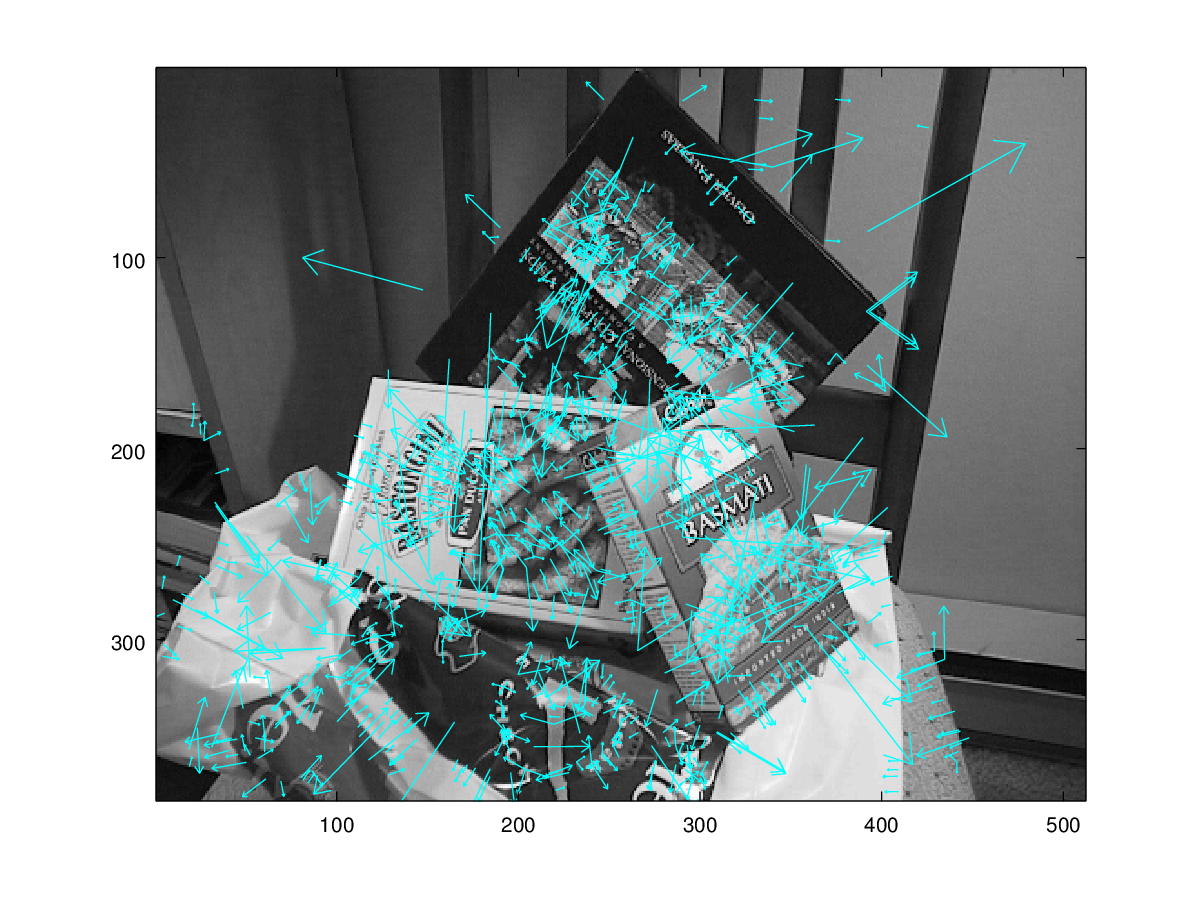
\includegraphics[width=0.9\textwidth]{./img/scene-keys.png} \\
\caption{The features SIFT finds in ``scene.pgm"}
\label{fig:scenekeys}
\end{figure}

The features SIFT finds in ``scene.pgm" are shown in Figure \ref{fig:scenekeys}.
Since SIFT uses the differences of gaussian pyramid technique, most keys can be found in regions where the intensities change.
These regions can be small or large depending on where in the pyramid it was found.
Running the \verb+whos+ command gives us the number of keys that are shown in this image, namely 1021 keys with 128 elements.
The SIFT paper mentions that the number of expected keys is in the order of thousands for a 512 by 512 pixel image.
Since our image is only 512 by 384 pixels, we can expect less.
Hence the number that we found is probably in agreement with the paper.
Also note that the number of elements in the keys are different from the paper, keys in the paper have 160 instead of 128 elements.
We assume the cause is that this implementation does not sample a higher plane in the image pyramid, since the difference in number of elements is in agreement with the number of samples taken in this plane.

\begin{figure}
\centering
    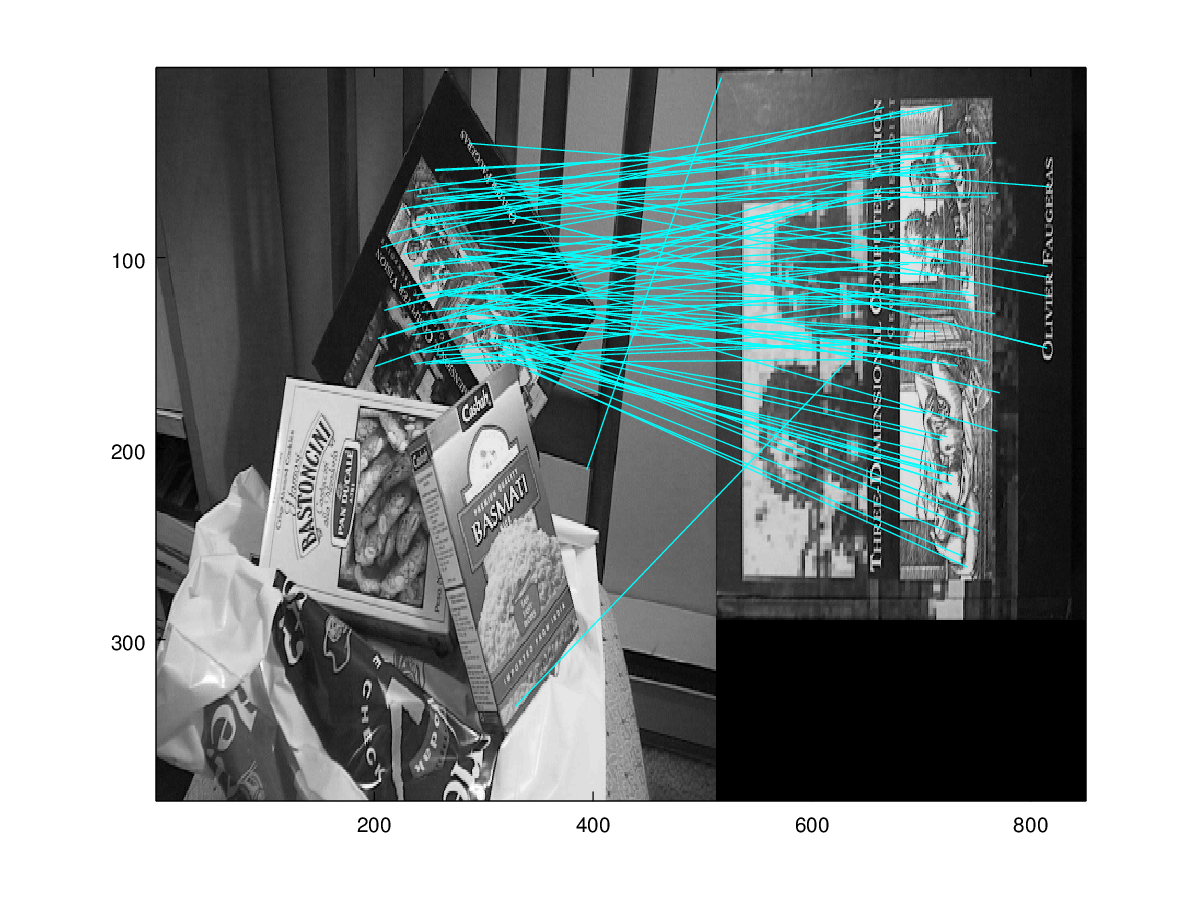
\includegraphics[width=0.9\textwidth]{./img/scene-book-match.png} \\
\caption{The matching features SIFT finds in ``scene.pgm" with ``book.pgm"}
\label{fig:scenebookmatch}
\end{figure}

The result of matching this scene with ``book.pgm" is shown in Figure \ref{fig:scenebookmatch}, it also shows the 98 matching keypoints with lines denoting matches.
This amounts to $9.5\%$ of the keypoints in ``scene.pgm" and $11\%$ of the keypoints in ``book.pgm".
It also shows two mismatches.
The first mismatch is between a corner from the book and a corner in the background of the scene.
The second one is between part of the bowl of rice and part of the image of the book.
It is understandable that these matches exist, since the features(colors/texture) are similar in the neighborhoods of the keypoints if you account for orientation.

\begin{figure}
\centering
    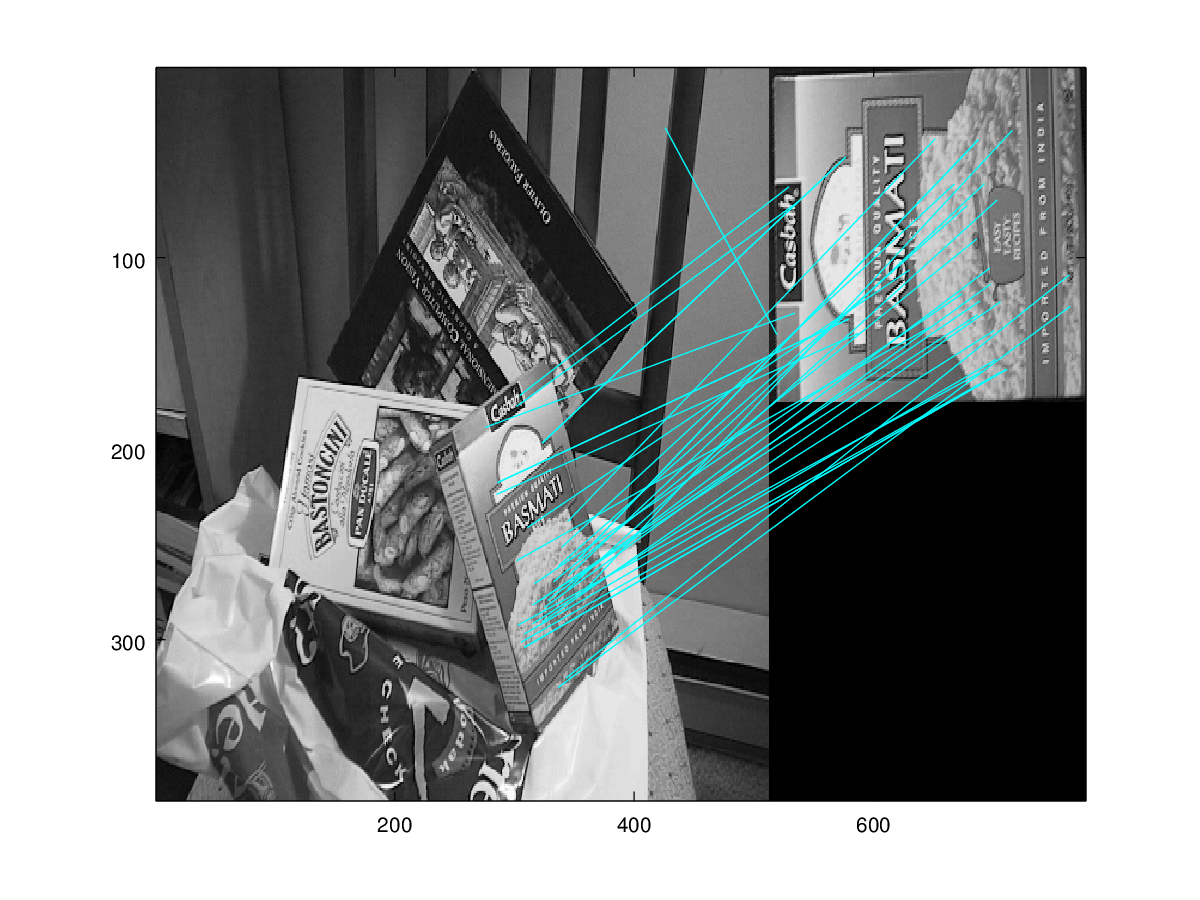
\includegraphics[width=0.9\textwidth]{./img/scene-basmati-match.png} \\
\caption{The matching features SIFT finds in ``scene.pgm" with ``basmati.pgm"}
\label{fig:scenebasmatimatch}
\end{figure}

The result of matching this scene with ``basmati.pgm" is shown in Figure \ref{fig:scenebasmatimatch}, it also shows the 34 matching keypoints with lines denoting matches.
This amounts to $3.3\%$ of the keypoints in ``scene.pgm" and $5.9\%$ of the keypoints in ``basmati.pgm".
Only one mismatch exists in this case between the edge in the background of the scene and the edge of the basmati box.
Again the mismatch is reasonable, since in the local neighborhoods of the matches are similar.
The other mismatch from the book case does not exist, because that part of the book is occluded in the scene.
Also note that in both case only a tiny percentage of the keys had to be matched in the scene to recognize the object.

\begin{figure}
\centering
\begin{tabular}{cc}
    Normal street image & Large street image \\
    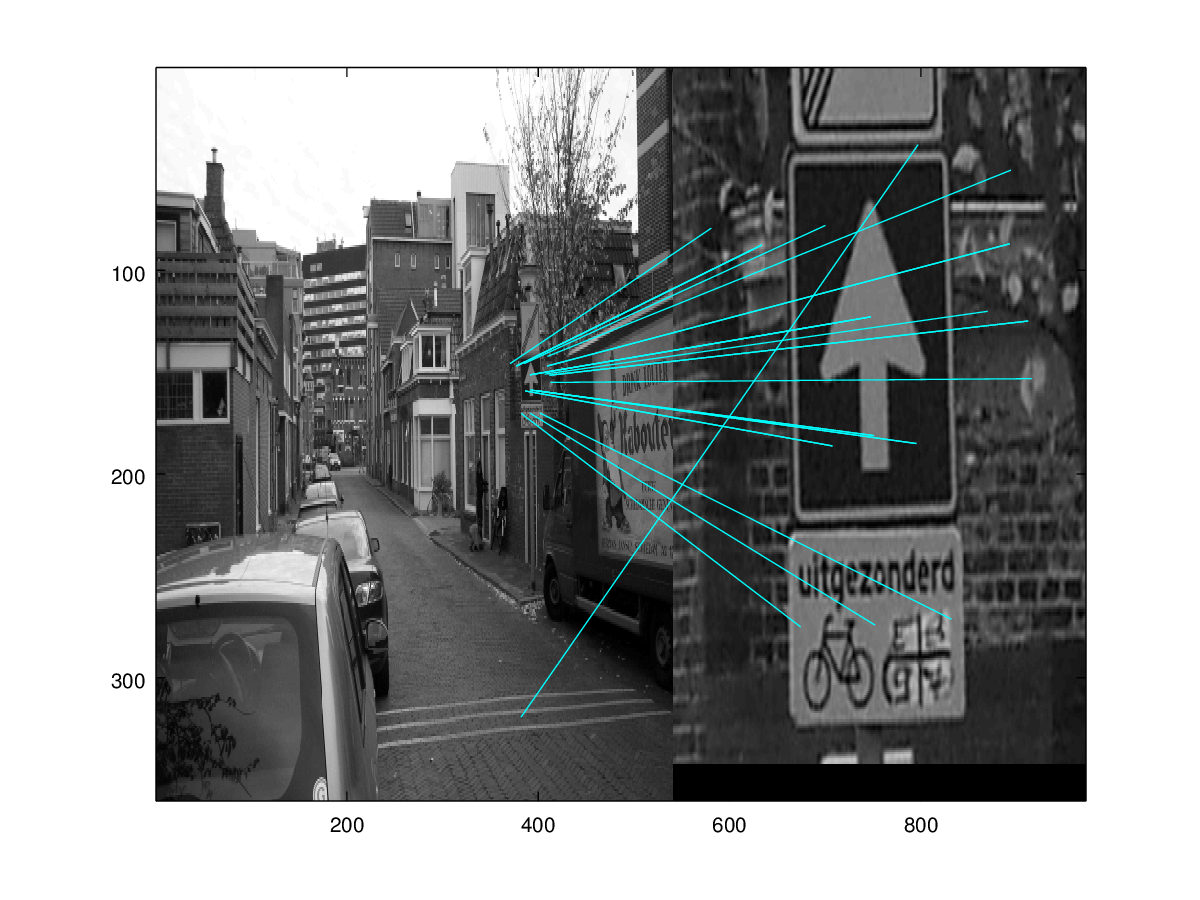
\includegraphics[width=0.45\textwidth]{./img/street-d1-match.png} & 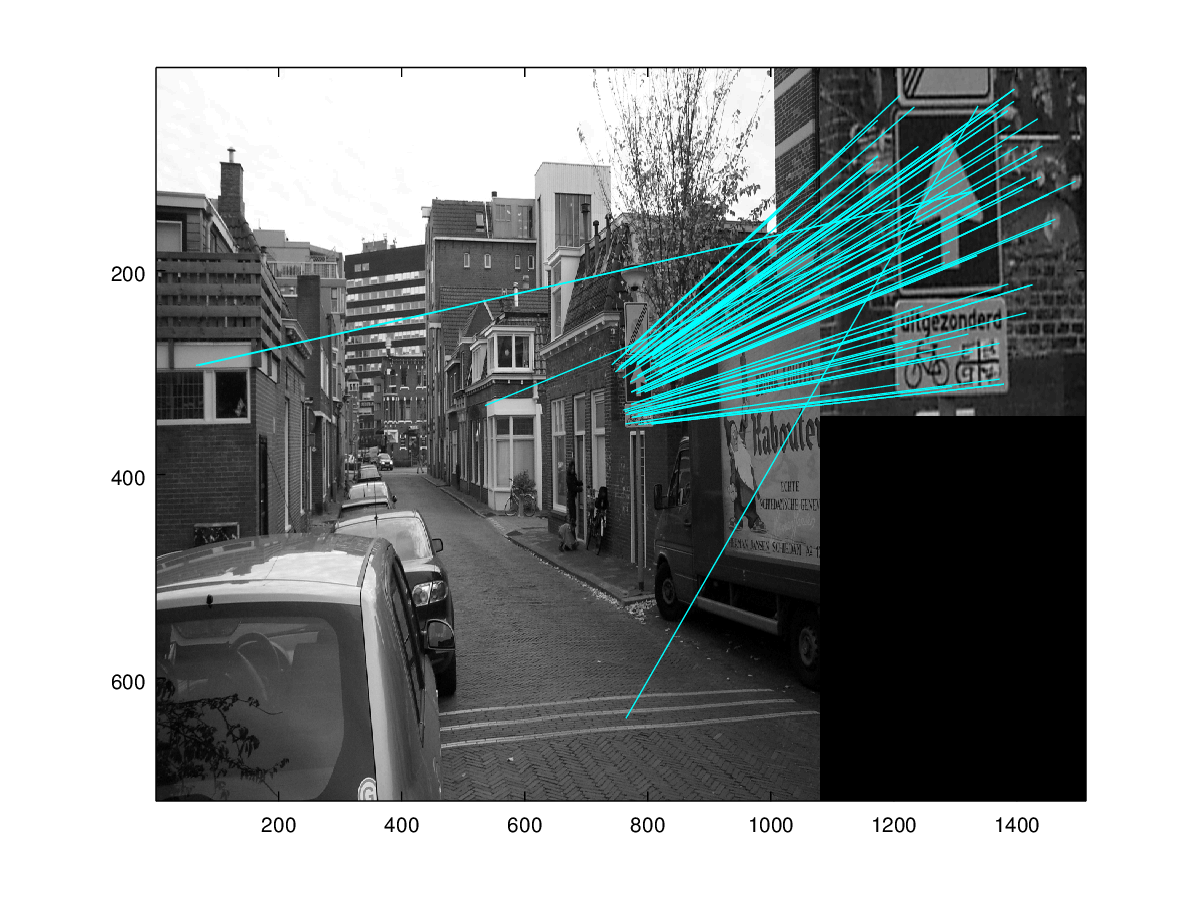
\includegraphics[width=0.45\textwidth]{./img/streetlarge-d1-match.png} \\
    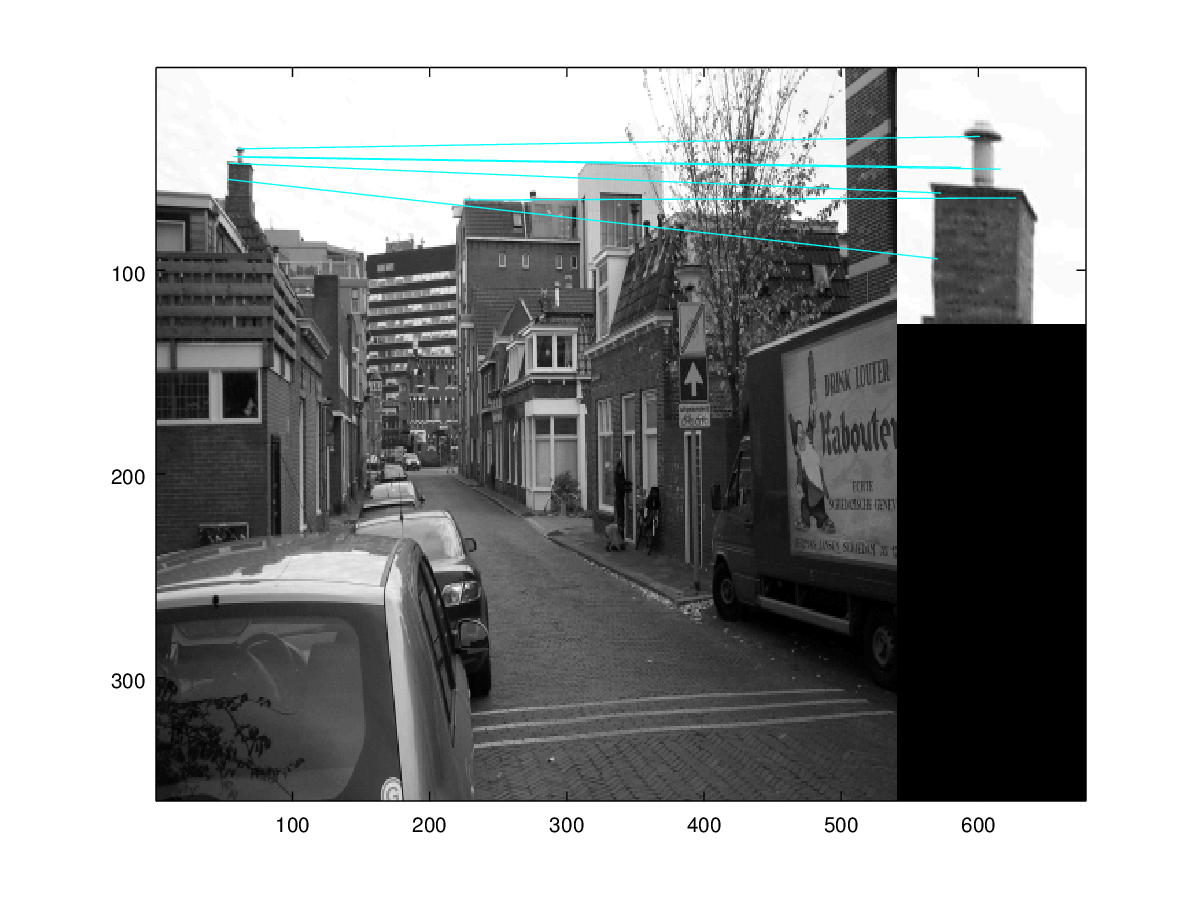
\includegraphics[width=0.45\textwidth]{./img/street-d2-match.png} & 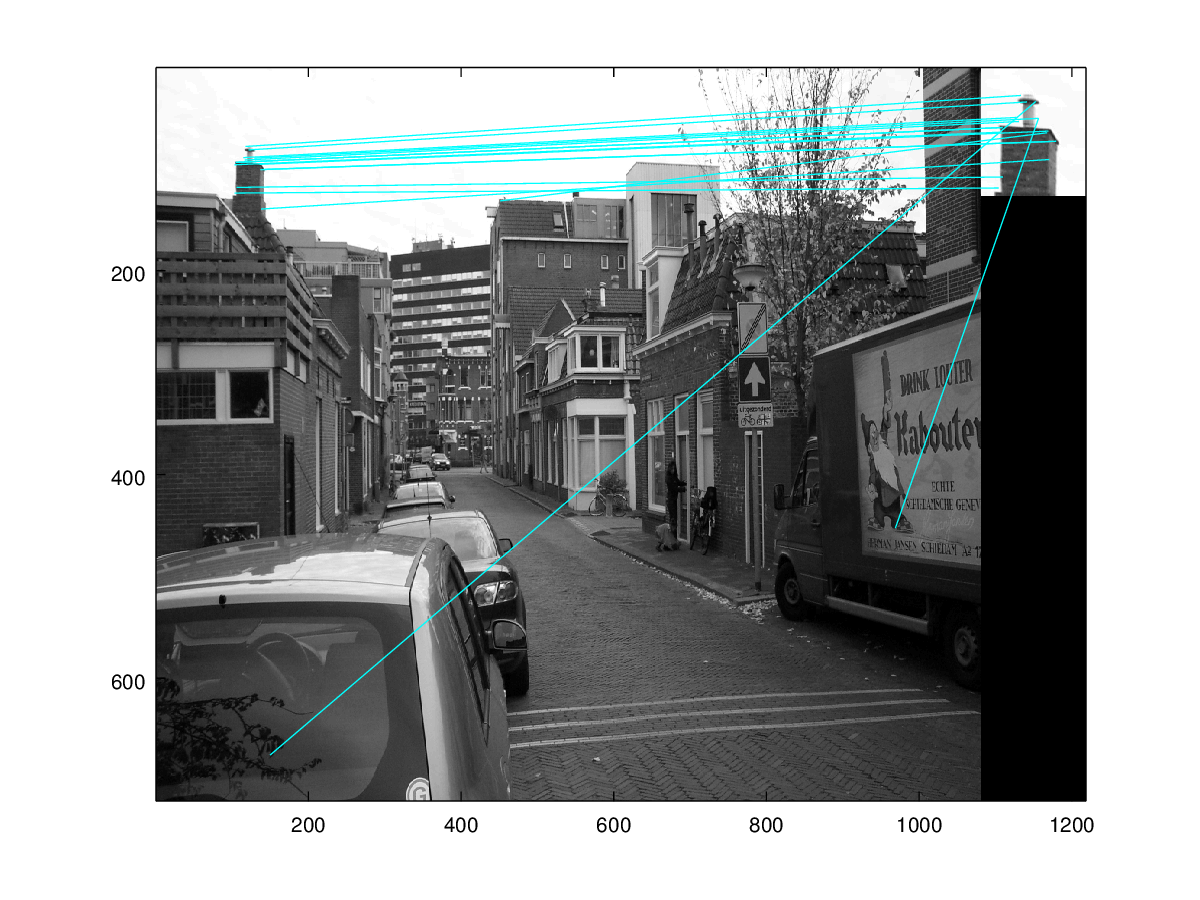
\includegraphics[width=0.45\textwidth]{./img/streetlarge-d2-match.png} \\
    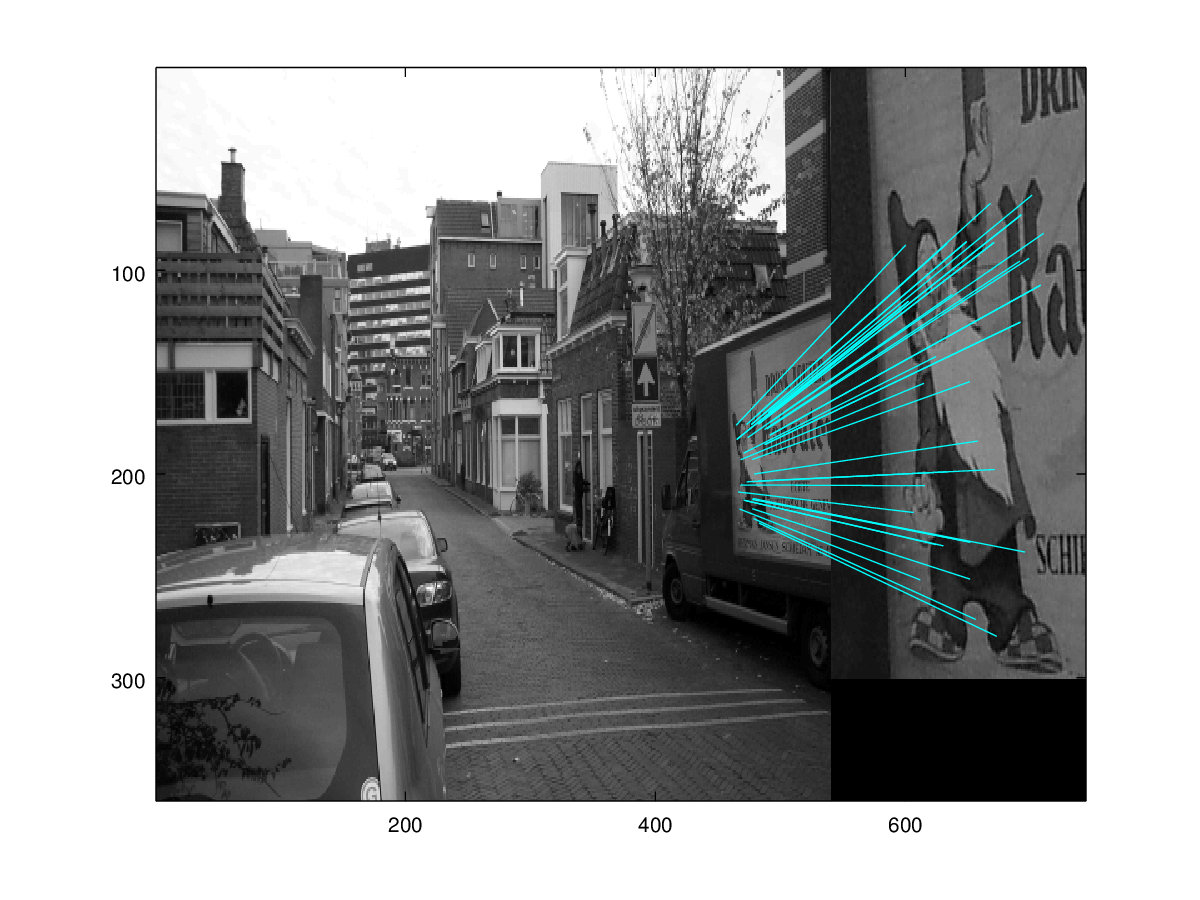
\includegraphics[width=0.45\textwidth]{./img/street-d3-match.png} & 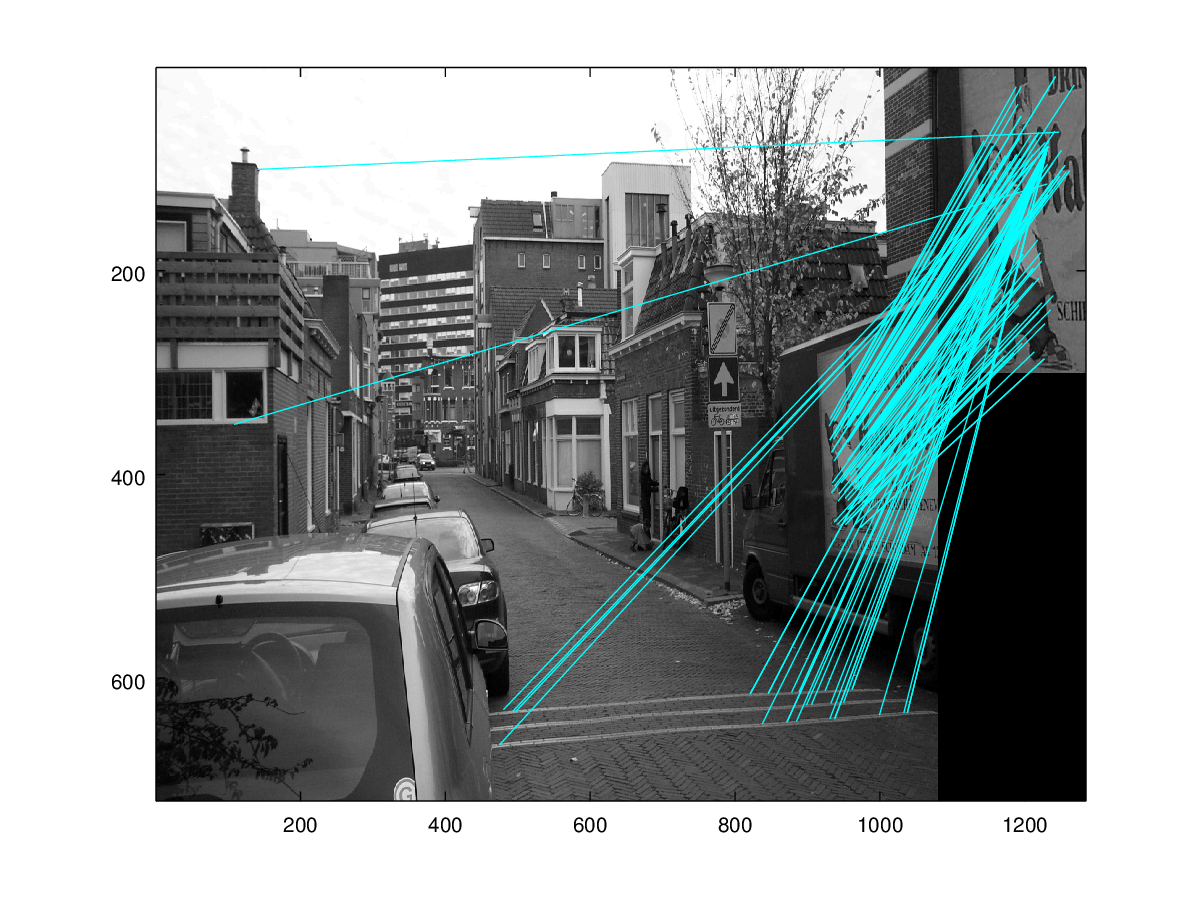
\includegraphics[width=0.45\textwidth]{./img/streetlarge-d3-match.png} \\
    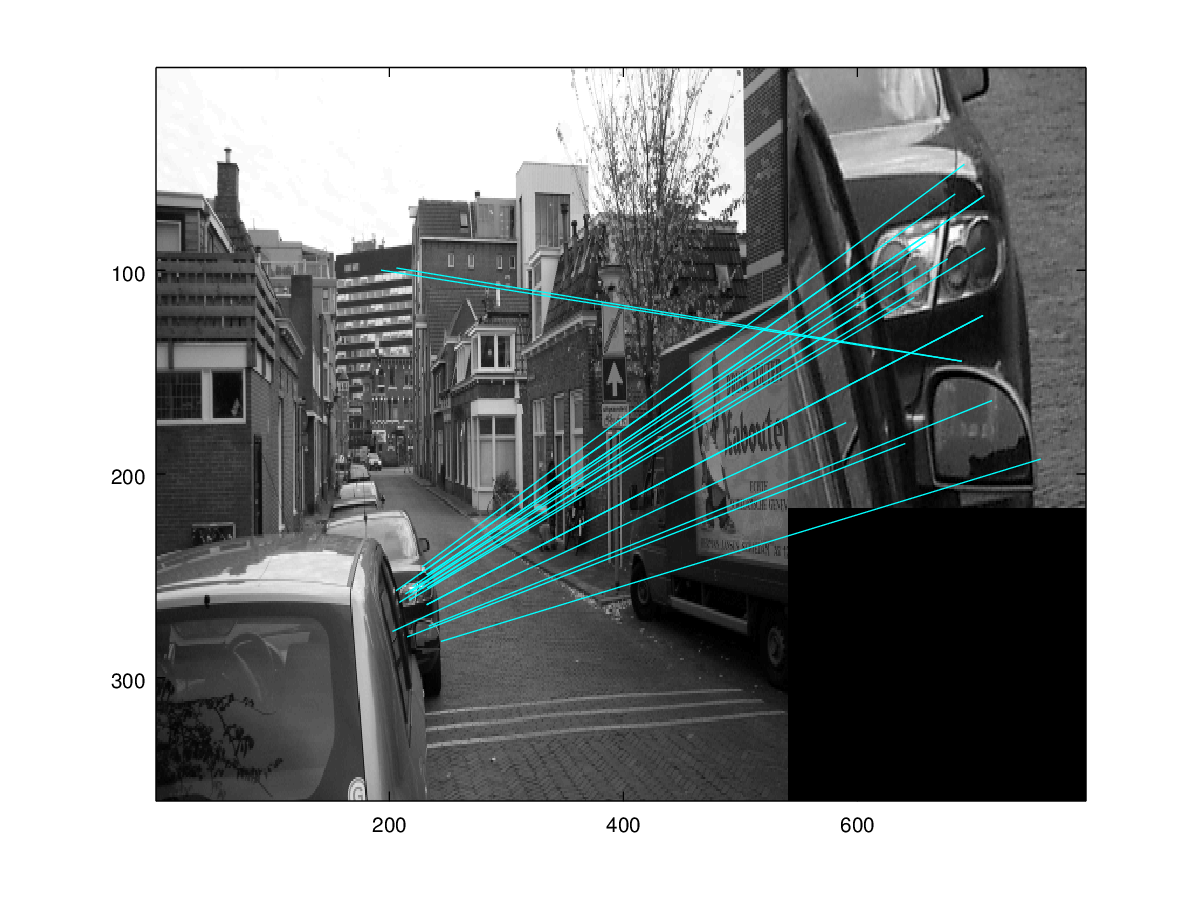
\includegraphics[width=0.45\textwidth]{./img/street-d4-match.png} & 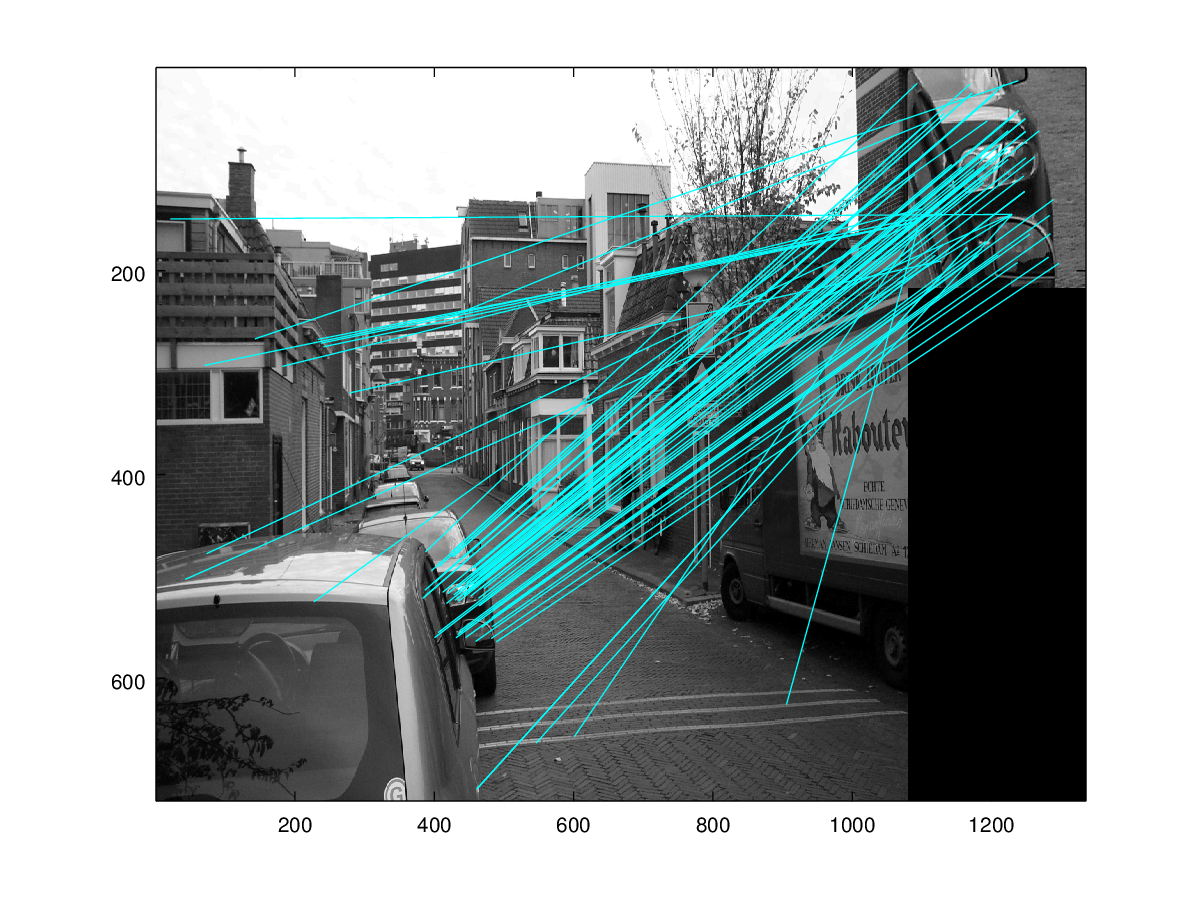
\includegraphics[width=0.45\textwidth]{./img/streetlarge-d4-match.png} \\
\end{tabular}
\caption{The SIFT matches of the street and large street scene with the detail 1 to 4 vertically images.}
\label{fig:streetdetails14}
\end{figure}

Let us consider the effect of the resolution of the scene images with respect to the matched objects.
Figure \ref{fig:streetdetails14} and \ref{fig:streetdetails5} show the results of SIFT matching.
As can be seen in the images the number of matches is higher, but the number of mismatches also increased.
If we ignore the mismatches for now, then we get that the number of matches increased approximately linearly with the number of keys in the scene image.
Table \ref{tab:streetdetails} shows the number of matches per image combination, while Table \ref{tab:streetkeys} lists the number of keys per image.
In this case the large image has about 3 to 4 times the amount of keys with respect to the normal image and the number of matches increased with a similar factor.

\begin{figure}
\centering
\begin{tabular}{c}
    Normal street image \\
    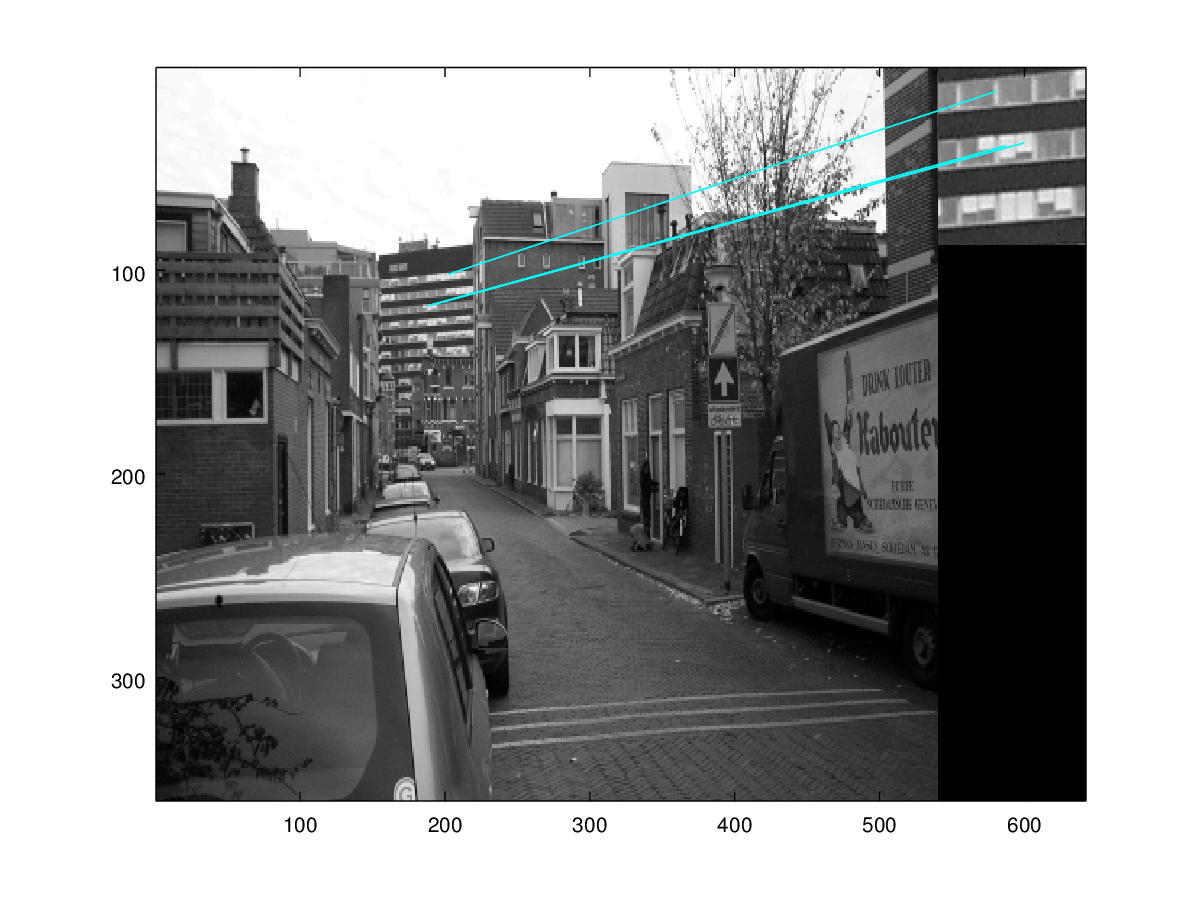
\includegraphics[width=0.9\textwidth]{./img/street-d5-match.png} \\
    Large street image \\
    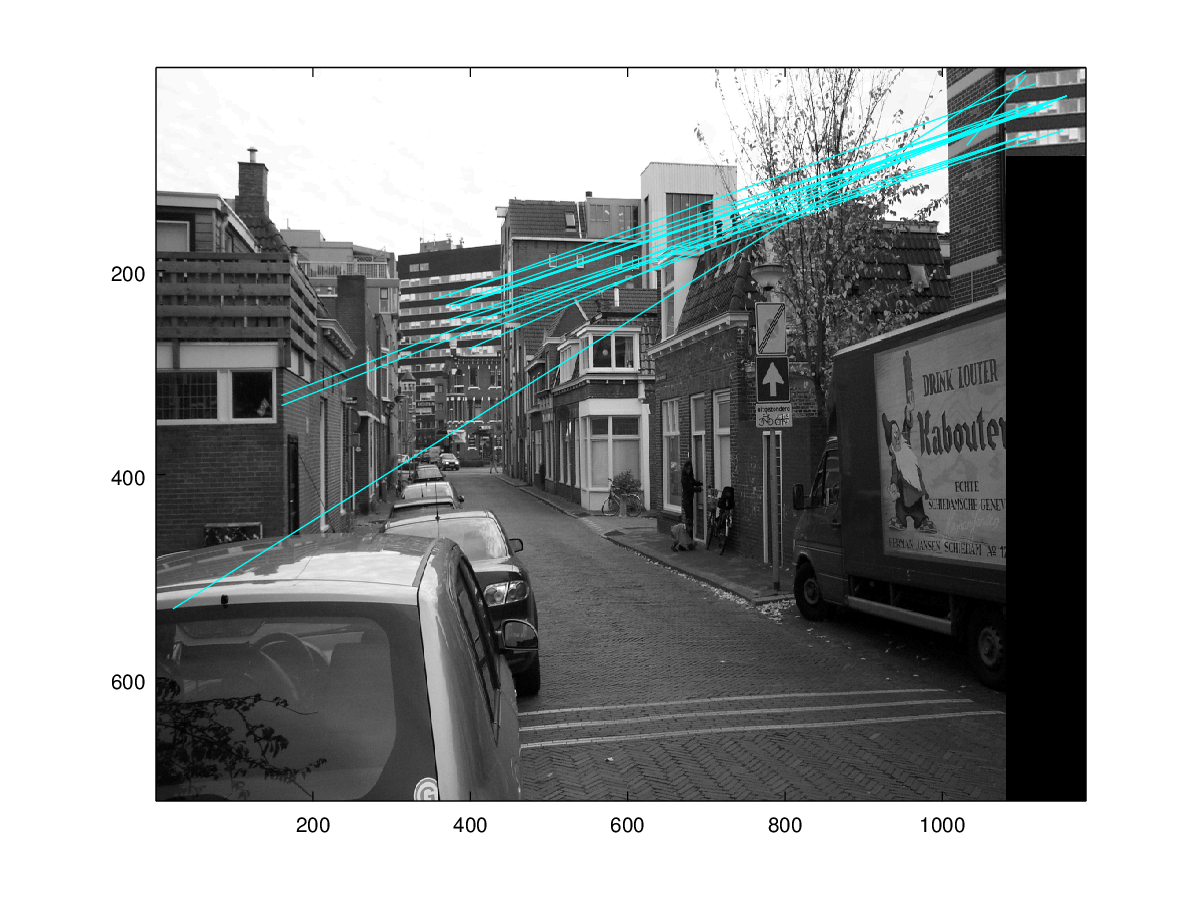
\includegraphics[width=0.9\textwidth]{./img/streetlarge-d5-match.png} \\
\end{tabular}
\caption{The SIFT matches of the street and large street scene with the detail 5 image.}
\label{fig:streetdetails5}
\end{figure}

The number of mismatches seems to be related to the number of keys of the object relative to the number of keys of the scene.
This is mainly based on the observation that in Figure \ref{fig:streetdetails14} and \ref{fig:streetdetails5} the larger street image seems to have more mismatches.
Object images that are about have the size of the scene image seem to do ok, but smaller ones have plenty of mismatches.
The extreme case is detail image 5 with the large street image, most of the matches are mismatches.
So having higher resolution one one image does not decrease the number of mismatches.

\begin{table}
    \centering
    \begin{tabular}{c|c|c|c|c|c|c}
        Street & Large street & Detail 1 & Detail 2 & Detail 3 & Detail 4 & Detail 5 \\
        \hline
        1452 & 5216 & 1592 & 46 & 588 & 368 & 126 \\
    \end{tabular}
    \caption{The number of keys per image.}
    \label{tab:streetkeys}
\end{table}

\begin{table}
    \centering
    \begin{tabular}{l|r|r|r|r|r|}
        & detail 1 & detail 2 & detail 3 & detail 4 & detail 5 \\
        \hline
        Street & 25 & 6 & 37 & 20 & 6 \\
        \hline
        Large street & 82 & 17 & 110 & 73 & 17 \\
        \hline
    \end{tabular}
    \caption{The number of matches between the different street scenes.}
    \label{tab:streetdetails}
\end{table}

\section*{Exercise 2}

\section*{Exercise 3}

Table \ref{tab:bookrotation} shows how the number of matches and the number of keys of the book changes with rotation.
The number of matches is rather stable.
This is good, because SIFT is supposed to be invariant to rotation.
Of course this does not mean that it is completely insensitive to rotation.
When sift samples the gradient it does so in a 4 by 4 grid with 8 different rotations thus generating 128 keys.
The also is the cause of the insensitivity to rotation.
The small fluctuations in the number of keys and matches is probably caused by how fitting the alignment is for detecting significant features.

\begin{table}[h]
    \centering
    \begin{tabular}{c|c|c}
        rotation (degrees) & \#matches & \#keys \\
        \hline
        0 & 98 & 882 \\
        \hline
        10 & 102 & 1020 \\
        \hline
        20 & 95 & 1016 \\
        \hline
        30 & 107 & 1031 \\
        \hline
        40 & 101 & 1055 \\
        \hline
        50 & 100 & 1055 \\
        \hline
        60 & 102 & 1053 \\
        \hline
        70 & 102 & 1019 \\
        \hline
        80 & 107 & 1042 \\
        \hline
        90 & 103 & 902 \\
        \hline
        180 & 98 & 907 \\
        \hline
        270 & 100 & 915 \\
    \end{tabular}
    \caption{The number of matches and keys of the book depending on the rotation.}
    \label{tab:bookrotation}
\end{table}



\section*{Exercise 4}

\end{document}
